\section{The method} \label{sec:method}

%%%%%%%%%%%%%%%%%%%%%%%%%%%%%%%%%%%%%%%%%%%%%%%%%%%%%%%%%%%%%%%%%%%%%%%%%%%%%%%%%%%%%%%%
\subsection{The $Q$ transform} \label{sec:method:qtransform}
To conduct the multi-resolution analysis motivated in the introduction, the data are processed using the $Q$ transform~\cite{Brown:1991}. The $Q$ transform is a modification of the standard short time Fourier transform in which the analysis window duration varies inversely with frequency such that the time-frequency plane is covered by tiles of constant quality factor $Q$. The signal time series, $x(t)$, is projected onto a basis of complex-valued windowed sine waves:
\begin{equation}
  X(\tau, \phi, Q) = \int_{-\infty}^{+\infty}{ x(t) w(t-\tau,\phi,Q) e^{-2i\pi\phi t}dt}.
  \label{eq:qtransform1}
\end{equation}
The transform coefficient, $X$, measures the average signal amplitude and phase within a time-frequency region, called a \textit{tile}, centered on time $\tau$ and frequency $\phi$, whose shape and area are determined by the requested quality factor $Q$ and the particular choice of analysis window, $w$. In~\cite{Gabor:1946}, it is shown that the minimal time-frequency resolution is achieved by a Gaussian window:
\begin{equation}
  w(t-\tau,\phi,Q) = \frac{W_g}{\sigma_t\sqrt{2\pi}}\exp\left [ -\frac{1}{2\sigma_t^2}(t-\tau)^2 \right],
  \label{eq:gausswindowt}
\end{equation}
where $W_g$ is a normalization factor and the Gaussian variance is $\sigma_t^2=\frac{Q^2}{8\pi^2\phi^2}$.

To optimize the algorithmic implementation of the $Q$ transform, we prefer an alternative form of Eq.~\ref{eq:qtransform1}, where we switch to the frequency domain using the Fourier transform defined as
\begin{equation}
  \tilde{x}(f) = \int_{-\infty}^{+\infty}{ x(t) e^{-2i\pi f t}dt}. \label{eq:FTforward}
\end{equation}
The corresponding reverse Fourier transform is
\begin{equation}
  x(t) = \int_{-\infty}^{+\infty}{ \tilde{x}(f) e^{2i\pi f t}df}.  \label{eq:FTbackward}
\end{equation}
Using the inverse Fourier transform, the cross-correlation theorem, the Fourier transform translation relation and the fact that we are working with a real window, we can re-write Eq~\ref{eq:qtransform1}:
\begin{align}
  X(\tau, \phi, Q) &= \int_{-\infty}^{+\infty}{\tilde{X}(f,\phi,Q) e^{+2i\pi f \tau}df} \\
  X(\tau, \phi, Q) &= \int_{-\infty}^{+\infty}{ \widetilde{\left (\int_{-\infty}^{+\infty}{w^*(t,\phi,Q)x(t+\tau)e^{-2i\pi\phi(t+\tau)}dt}\right)} e^{+2i\pi f \tau}df}\\
  X(\tau, \phi, Q) &= \int_{-\infty}^{+\infty}{ \tilde{x}(f+\phi) \tilde{w}^{*}(f,\phi,Q) e^{+2i\pi f \tau}df}.
  \label{eq:qtransform2}
\end{align}
In Eq.~\ref{eq:qtransform2}, the signal is applied a Fourier transform, a shift in frequency, a multiplication by the frequency-domain window and an inverse Fourier transform.


%%%%%%%%%%%%%%%%%%%%%%%%%%%%%%%%%%%%%%%%%%%%%%%%%%%%%%%%%%%%%%%%%%%%%%%%%%%%%%%%%%%%%%%%
\subsection{The window} \label{sec:method:window}
To compute the $Q$ transform of Eq.~\ref{eq:qtransform2}, we need to apply a Fourier transform to the Gaussian window of Eq.~\ref{eq:gausswindowt}. In the frequency domain, the window is also Gaussian and real:
\begin{equation}
  \tilde{w}(f,\phi,Q) = \tilde{w}^*(f,\phi,Q) = W_g\exp\left [ -\frac{1}{2\sigma_f^2}f^2 \right],
  \label{eq:gausswindowf}
\end{equation}
where $\sigma_f^2=\frac{2\phi^2}{Q^2}$.

The Gaussian window provides the best time-frequency resolution~\cite{Gabor:1946}. However, such a window has an infinite extent which makes it difficult to use in a discrete analysis framework. Instead, the Omicron algorithm approximates the Gaussian window with a bisquare window which has a simple form in the frequency domain:
\begin{equation}
  \tilde{w}(f,\phi,Q) = \tilde{w}^*(f,\phi,Q) =
  \begin{cases}
    W_b\left[1 - \left(\frac{f}{\delta_f(\phi,Q)}\right)^2 \right]^2 & |f| < \delta_f(\phi,Q), \\
    0 & \textrm{otherwise},
  \end{cases}
  \label{eq:bisquare}
\end{equation}
where $W_b$ is a normalization factor and $\delta_f(\phi,Q)=\phi\sqrt{11}/Q$ is the half size of the window. This window is a very good approximation to the Gaussian case~\cite{Chatterji:2004}. It achieves a time-frequency resolution that is only 4.5~\% greater than the minimum possible time-frequency uncertainty associated with the ideal Gaussian window. In addition, it offers a limited energy leakage into time-domain side lobes.

Thanks to the finite extent of the the bisquare window, it is possible to add protections against signal aliasing. Indeed, when using the two conditions
\begin{align}
  &Q\ge\sqrt{11} \qquad \text{and}\label{eq:antialias1} \\
  &\phi \le \frac{f_{\text{Nyquist}}}{1+\sqrt{11}/Q}, \label{eq:antialias2}
\end{align}
the zero frequency and the Nyquist frequency, $f_{\text{Nyquist}}$, are never exceeded: $0 \le f + \phi \le f_{\text{Nyquist}}$. The $Q$ transform in Eq.~\ref{eq:qtransform2} can, therefore, be safely discretized as we will see in Sec.~\ref{sec:algorithm:projection}.

The window normalization factor is such that
\begin{equation}
  \int_{-\infty}^{+\infty}{|\tilde{w}(f,\phi,Q)|^2df} = 2.
  \label{eq:winnorm}
\end{equation}
Using this normalization condition has many advantages which will be presented in Sec.~\ref{sec:method:snr}. A trivial integration yields the normalization factor for the bisquare window
\begin{equation}
  W_b = \sqrt{\frac{315}{128\sqrt{11}} \frac{Q}{\phi}},
  \label{eq:Wb}
\end{equation}
while for the Gaussian case we get
\begin{equation}
  W_g = \sqrt{\frac{2}{\sqrt{\pi}\sigma_f}} = \sqrt{\sqrt{\frac{2}{\pi}} \frac{Q}{\phi}},
  \label{eq:Wg}
\end{equation}

A characteristic duration, $\Delta t$, and bandwidth, $\Delta f$, are defined using the second central moments of the window:
\begin{align}
  \left(\frac{\Delta f}{2}\right)^2 &= \int_{-\infty}^{+\infty}{f^2|\tilde{w}(f,\phi,Q)|^2 df}\\
  \left(\frac{\Delta t}{2}\right)^2 &= \int_{-\infty}^{+\infty}{t^2|w(t,\phi,Q)|^2 dt}.
\end{align}
For both the Gaussian and bisquare windows, we naturally find indentical values:
\begin{align}
  \Delta f &=  2\sigma_f = 2\sqrt{2}\frac{\phi}{Q}, \\ 
  \Delta t &=  2\sigma_t = \frac{1}{\sqrt{2}\pi}\frac{Q}{\phi}.
\end{align}
Fig.~\ref{fig:window} shows a comparison between an ideal Gaussian window and its approximate using a bisquare window.
\begin{figure}
  \center
  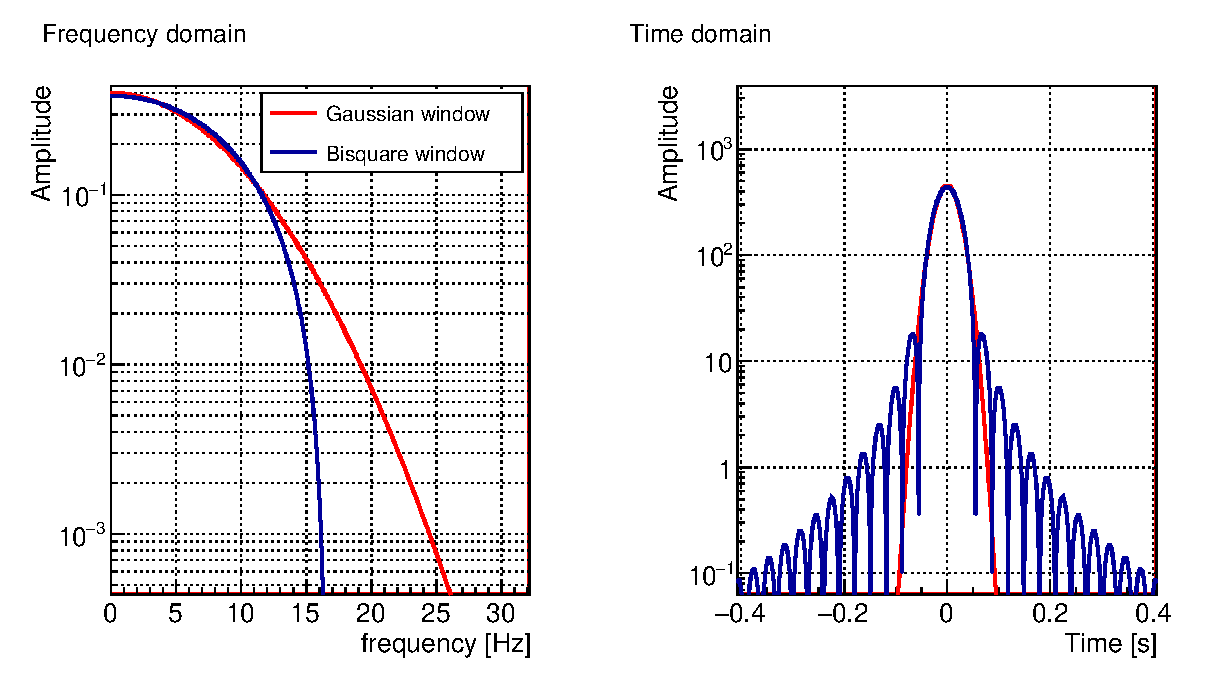
\epsfig{width=12cm, file=./figures/window.eps}
  \caption{A Gaussian window (red) is approximated by a bisquare window (blue) in the frequency domain (left) and, after an inverse Fourier transform, in the time domain (right). We used $\phi=100$~Hz and $Q=20$.}
  \label{fig:window}
\end{figure}

In the following, we will often refer to a basis of complex-valued sinusoidal Gaussian waveforms keeping in mind that bisquare windows are actually used for the Omicron implementation.


%%%%%%%%%%%%%%%%%%%%%%%%%%%%%%%%%%%%%%%%%%%%%%%%%%%%%%%%%%%%%%%%%%%%%%%%%%%%%%%%%%%%%%%%
\subsection{The tiles} \label{sec:method:tiles}
The tiles must be chosen to cover a finite region of parameter space, $[\tau_{min};\tau_{max}]\times [\phi_{min};\phi_{max}] \times [Q_{min};Q_{max}]$. The density of tiles must be large to guarantee a high detection efficiency. However, the number of tiles must also be as small as possible to provide a fast processing. To meet these two competitive requirements, the parameter space is tiled such that the fractional energy loss due to mismatch is below a pre-defined value, $\mu_{max}$. For complex-valued sinusoidal Gaussian waveforms, the mismatch can be analytically computed and the optimal number of tiles can be determined. The Omicron algorithm adopts the tiling strategy developed in~\cite{Chatterji:2004}, where the tiles are distributed over a cubic lattice using a mismatch metric\footnote{The metric includes a non-diagonal $\delta \phi \delta Q$ term which has been neglected.} to measure distances:
\begin{equation}
  \delta s^2 =
  \frac{4\pi^2\phi^2}{Q^2}\delta \tau^2
  + \frac{2+Q^2}{4\phi^2}\delta \phi^2
  + \frac{1}{2Q^2}\delta Q^2.
  \label{eq:tilemetric}
\end{equation}
To guarantee a fractional energy loss smaller than $\mu_{max}$, the minimum number of tiles, $N_\tau \times N_\phi \times N_Q$, is given by the mismatch distances integrated over the three dimensions:
\begin{align}
  N_\tau \ge \frac{s_\tau}{2\sqrt{\mu_{max}/3}},  & \qquad s_\tau = \frac{2\pi\phi}{Q}(\tau_{max} - \tau_{min}), \label{eq:tiledistancetau} \\
  N_\phi \ge \frac{s_\phi}{2\sqrt{\mu_{max}/3}},  & \qquad s_\phi = \frac{\sqrt{2+Q^2}}{2}\ln(\phi_{max}/\phi_{min}), \label{eq:tiledistancephi} \\
  N_Q \ge \frac{s_Q}{2\sqrt{\mu_{max}/3}},  & \qquad s_Q = \frac{1}{\sqrt{2}}\ln(Q_{max}/Q_{min}). \label{eq:tiledistanceq}
\end{align}
This Omicron tiling structure can be depicted as a set of $N_Q$ logarithmically-spaced $Q$ planes, indexed by $q$:
\begin{equation}
  Q_q = Q_{min}\left[ \frac{Q_{max}}{Q_{min}}\right]^{(0.5+q)/N_q}, \qquad 0\le q < N_Q.
  \label{eq:q}
\end{equation}
Each of these planes is divided into $N_\phi(Q_q)$ logarithmically-spaced frequency rows, indexed by $q$ and $l$:
\begin{equation}
  \phi_{ql} = \phi_{min}\left[ \frac{\phi_{max}}{\phi_{min}}\right]^{(0.5+l)/N_\phi(Q_q)}, \qquad 0\le l < N_\phi(Q_q).
  \label{eq:phi}
\end{equation}
Each frequency row is finally sub-divided into $N_\tau(Q_q,\phi_{ql})$ linearly-spaced time bins, indexed by $q$, $l$ and $m$:
\begin{equation}
  \tau_{qlm} = \tau_{min}+(m+0.5)\frac{\tau_{max}-\tau_{min}}{N_\tau(Q_q,\phi_{ql})}, \qquad 0\le m < N_\tau(Q_q,\phi_{ql}).
  \label{eq:tau}
\end{equation}


%%%%%%%%%%%%%%%%%%%%%%%%%%%%%%%%%%%%%%%%%%%%%%%%%%%%%%%%%%%%%%%%%%%%%%%%%%%%%%%%%%%%%%%%
\subsection{The noise whitening} \label{sec:method:whitening}

As we will see in Sec.~\ref{sec:method:snr}, whitening the noise before applying the $Q$ transform is useful for a subsequent statistical interpretation of the $Q$ transform coefficients. To achieve this, a simple method consists of re-weighting the frequency-domain data by the inverse noise amplitude spectral density:
\begin{equation}
  \tilde{x}^{white}(f) = \frac{\tilde{x}(f)}{\sqrt{S_n(|f|)/2}},
  \label{eq:whitening}
\end{equation}
where $S_n(f)$ is the one-sided ($f \ge 0$) noise power spectrum density (PSD). After this transformation, the power of a random noise process is equally distributed over the frequencies and the one-sided PSD of $x^{white}$ is flat and equal to 2.

The noise one-sided PSD is usually estimated by averaging multiple one-sided periodograms computed over a finite duration $T$ (Welch method):
\begin{equation}
  P_T(f) = \frac{2}{T}\left|\tilde{x}_T(f)\right|^2, \qquad f \ge 0.
  \label{eq:periodogram}
\end{equation}
In a one-sided convention, the factor 2 accounts for the negative frequencies of $\tilde{x}_T$. Note that this factor is corrected back when whitening the data in Eq.~\ref{eq:whitening}.


%%%%%%%%%%%%%%%%%%%%%%%%%%%%%%%%%%%%%%%%%%%%%%%%%%%%%%%%%%%%%%%%%%%%%%%%%%%%%%%%%%%%%%%%
\subsection{The signal to noise ratio} \label{sec:method:snr}

Let's consider a burst of energy, the waveform of which is $b(t)$. It lies on top of noise, $n(t)$, such as $x(t) = b(t) + n(t)$. An amplitude $Q$ transform signal-to-noise ratio (SNR) for each tile is defined as
\begin{equation}
  \rho_{qlm}^2 =  \frac{|X_b(\tau_{qlm}, \phi_{ql}, Q_q)|^2}{\langle |X_n(\tau_{qlm}, \phi_{ql}, Q_q)|^2 \rangle/2}, \label{eq:snrdef}
\end{equation}
where $X_b(\tau_{qlm}, \phi_{ql}, Q_q)$ is the $Q$ transform coefficient for the burst waveform in tile $(q,l,m)$. The expectation value of the $Q$ transform energies for noise in tile $(q,l,m)$, obtained from multiple measurements, is given by $\langle |X_n(\tau_{qlm}, \phi_{ql}, Q_q)|^2\rangle$.

The SNR definition given by Eq.~\ref{eq:snrdef} is consistent with the maximum achievable SNR defined in the framework of the matched filter theory~\cite{helstrom:1968}. To demonstrate this, let's consider a burst test signal exactly matching the tile under consideration. The burst waveform is a sinusoidal Gaussian function of time, the parameters of which match the tile $(q,l,m)$:
\begin{align}
  b(t) &= Bw(t-\tau_{qlm}, \phi_{ql}, Q_q)\cos(2\pi\phi_{ql} t + \theta_{bt}),\\
  \tilde{b}(f) &= \frac{B}{2}e^{-2i\pi f\tau_{qlm}}\left[ \tilde{w}(f-\phi_{ql},\phi_{ql},Q_q)e^{-2i\pi\tau_{qlm}(f-\phi_{ql})}e^{i\theta_{bt}}+\tilde{w}(f+\phi_{ql},\phi_{ql},Q_q)e^{-2i\pi\tau_{qlm}(f+\phi_{ql})}e^{-i\theta_{bt}}\right],
\end{align}
where $B$ is the signal amplitude and $\theta_{bt}$ is the arbitrary phase between the burst and the tile. Using the frequency-domain $Q$ transform of Eq.~\ref{eq:qtransform2}, we compute the squared magnitude of the $Q$ transform coefficient, or energy, for tile $(q,l,m)$:
\begin{align}
  |X_b(\tau_{qlm}, \phi_{ql}, Q_q)|^2 &= \left|\int_{-\infty}^{+\infty}{ \frac{B}{2}\left[ \tilde{w}(f,\phi_{ql},Q_q)+\tilde{w}(f+2\phi_{ql},\phi_{ql},Q_q)\right] \tilde{w}^{*}(f,\phi_{ql},Q_q) df} \right|^2\\
  &= \left|\int_{-\infty}^{+\infty}{ \frac{B}{2} \tilde{w}(f,\phi_{ql},Q_q) \tilde{w}^{*}(f,\phi_{ql},Q_q) df}\right|^2 \\
  &= B^2,
  \label{eq:qtransform_signal}
\end{align}
where we used the window normalization of~Eq.\ref{eq:winnorm} and the fact that $\tilde{w}^{*}(f,\phi_b,Q_b)\tilde{w}(f+2\phi_b,\phi_b,Q_b)=0$ if we use the bisquare window approximation verifying condition~\ref{eq:antialias1}.

Now, let's estimate the mean squared magnitude of the $Q$ transform coefficient for the noise in the denominator of Eq.~\ref{eq:snrdef}. We assume that the noise, $n(t)$, is a stationary stochastic process. With this assumption, the expectation value $\langle |X_n(\tau_{qlm}, \phi_{ql}, Q_q)|^2 \rangle$ is time-independent and the $\tau$ dependency can be dropped:
\begin{equation}
  \langle |X_n(\tau_{qlm}, \phi_{ql}, Q_q)|^2 \rangle = \langle |X_n(\phi_{ql}, Q_q)|^2 \rangle = \int_{-\infty}^{+\infty}{ \int_{-\infty}^{+\infty}{ \langle n(t)n^*(t') \rangle w(t,\phi_{ql},Q_q) w^*(t',\phi_{ql},Q_q) e^{-2i\pi\phi_{ql}(t-t')}dt}dt'}.
  \label{eq:qtransform_noise1}
\end{equation}
Then we can use the Wiener-Khinchin theorem, defining the one-sided power spectrum density of a stationary noise process,
\begin{equation}
  S_n(f)=2\int_{-\infty}^{+\infty}{ \langle n(t)n^*(t-T) \rangle e^{-2i\pi fT}dT},\qquad f\ge0
\end{equation}
and the autocorrelation theorem,
\begin{equation}
  \int_{-\infty}^{+\infty}{w(t)w^*(t-T)dt} = \int_{-\infty}^{+\infty}{|\tilde{w}(f)|^2e^{2i\pi fT}df},
\end{equation}
to re-write Eq.~\ref{eq:qtransform_noise1}:
\begin{equation}
  \langle |X_n(\tau_{qlm}, \phi_{ql}, Q_q)|^2 \rangle =  \frac{1}{2}\int_{-\infty}^{+\infty}{ |\tilde{w}(\phi_{ql}-f,\phi_{ql},Q_q)|^2S_n(|f|) df }.
  \label{eq:qtransform_noise}
\end{equation}
Taking into account the normalization condition~\ref{eq:winnorm}, the mean squared magnitude of the $Q$ transform coefficient for a stationary stochastic process can be interpreted as the noise power density integrated over the tile frequency window. Moreover, if we consider that the power spectral density is approximately constant over the window bandwidth, we get $\langle |X_n(\tau_{qlm}, \phi_{ql}, Q_q)|^2 \rangle \simeq S_n(\phi_{ql})$. This result, combined with Eq.~\ref{eq:qtransform_signal}, can be used to derive the SNR defined by Eq.~\ref{eq:snrdef}:
\begin{equation}
  \rho_{qlm} \simeq  \frac{B}{\sqrt{S_n(\phi_{ql})/2}}.
  \label{eq:snrmatch}
\end{equation}
As previously announced, this result is exactly what is obtained in the context of the matched filtering theory~\cite{helstrom:1968}. The factor 2 is used to correct for the power of negative frequencies folded in the one-sided PSD.

One must recall that the $Q$ transform is performed after whitening the time series as described in Sec.~\ref{sec:method:whitening}. The above calculation must therefore be modified. In particular, Eq.~\ref{eq:qtransform_signal} and Eq.~\ref{eq:qtransform_noise} become:
\begin{align}
  |X^{white}_b(\tau_{qlm}, \phi_{ql}, Q_q)| &= B \int_{-\infty}^{+\infty}{\frac{|\tilde{w}(f-\phi_{ql},\phi_{ql},Q_q)|^2}{2\sqrt{S_n(|f|)/2}}df}, \\
  \langle |X^{white}_n(\tau_{qlm}, \phi_{ql}, Q_q)|^2 \rangle &= 2.
  \label{eq:qtransform_whitened}
\end{align}
The SNR is then given by
\begin{equation}
  \rho_{qlm} = |X^{white}_b(\tau_{qlm}, \phi_{ql}, Q_q)| = B \int_{-\infty}^{+\infty}{\frac{|\tilde{w}(f-\phi_{ql},\phi_{ql},Q_q)|^2}{2\sqrt{S_n(|f|)/2}}df},
  \label{eq:snr_white}
\end{equation}
and the special case of Eq.~\ref{eq:snrmatch} remains true.

~

For obvious reasons, the burst signal cannot be disentangled from noise; only $x$ is measured. As a result, the SNR of Eq.~\ref{eq:snrdef} cannot be exactly computed. Instead, it is estimated using the $Q$ transform coefficient of $x$:
\begin{equation}
  \hat{\rho}_{qlm}^2 =  |X^{white}(\tau_{qlm}, \phi_{ql}, Q_q)|^2-2 . \label{eq:snrestimator}
\end{equation}
%To estimate the denominator, we rely, once more, on the noise stationarity hypothesis. The expectation value for noise can be evaluated using tiles at different times where we know that no burst signal is present, i.e. $x(t)=n(t)$. We note $\cal{T}$ such a representative set of tiles such as $\langle |X_n(\tau_{qlm}, \phi_{ql}, Q_q)|^2 \rangle = \langle |X_n(\phi_{ql}, Q_q)|^2 \rangle = \langle |X(\tau_{qli}, \phi_{ql}, Q_q)|^2 \rangle_{i\in \cal{T}}$. In Sec.~\ref{sec:algorithm:snr}, we will describe how the set $\cal{T}$ can be constructed.
The squared magnitude of the $Q$ transform coefficient of $x=b+n$ for tile $(q,l,m)$ can be expanded as
\begin{equation}
  |X(\tau_{qlm}, \phi_{ql}, Q_q)|^2 = |X_b(\tau_{qlm}, \phi_{ql}, Q_q)|^2 + |X_n(\tau_{qlm}, \phi_{ql}, Q_q)|^2 + 2|X_n(\tau_{qlm}, \phi_{ql}, Q_q)|\ |X_b(\tau_{qlm}, \phi_{ql}, Q_q)|\cos{\theta_{bn}},
\end{equation}
where $\theta_{bn}$ is the phase between the burst and the noise signals. Using this expression, and switching to whitened quantities, the SNR estimator can be re-written as
\begin{equation}
  \hat{\rho}_{qlm}^2  =
  \rho_{qlm}^2
  + |X^{white}_n(\tau_{qlm}, \phi_{ql}, Q_q)|^2 -2
  + 2|X^{white}_n(\tau_{qlm}, \phi_{ql}, Q_q)|\ |X^{white}_b(\tau_{qlm}, \phi_{ql}, Q_q)| \cos{\theta_{bn}}.
\end{equation}
From this expression, we see that our SNR estimate can differ from the true value because of two causes: the random fluctuations of white noise around the mean value of 2 and the arbitrary phase, $\theta_{bn}$, between the burst and the noise signals. Both distributions are known. In~\cite{Chatterji:2004}, it is shown that the distribution of $|X^{white}_n(\tau_{qlm}, \phi_{ql}, Q_q)|^2$ is an exponential distribution with mean $\langle |X^{white}_n(\tau_{qlm}, \phi_{ql}, Q_q)|^2 \rangle = 2$. The standard deviation of $|X^{white}_n(\tau_{qlm}, \phi_{ql}, Q_q)|^2$ from 2 is therefore 2. In addition, assuming that the signal and the noise are independent, the distribution of the phase $\theta_{bn}$ is uniform over all angles. One additional source of uncertainty result from the assumption made until now: the match between the burst signal and the tile is never perfect. However it can be improved by using a finer tiling structure as described in Sec.~\ref{sec:method:tiles} and this effect can be neglected when working with a low maximum mismatch value ($\mu_{max}$).


%%%%%%%%%%%%%%%%%%%%%%%%%%%%%%%%%%%%%%%%%%%%%%%%%%%%%%%%%%%%%%%%%%%%%%%%%%%%%%%%%%%%%%%%
\subsection{The signal amplitude and phase} \label{sec:method:ampphase}

The SNR expression in Eq.~\ref{eq:snr_white} suggests that it is possible to estimate the signal amplitude:
\begin{equation}
  \hat{B} = \frac{\hat{\rho}_{qlm}}{\int_{-\infty}^{+\infty}{\frac{|\tilde{w}(f-\phi_{ql},\phi_{ql},Q_q)|^2}{2\sqrt{(S_n(|f|)/2)}}df}}.
  \label{eq:amplitude}
\end{equation}
By construction, this estimate of the amplitude differ from the true amplitude value for the same reasons listed in the previous section. Moreover, this amplitude only reflects how a given signal projects on a sinusoidal Gaussian waveform.

 \bluenote{What about the phase?}
